\documentclass[letterpaper,12pt]{article}

% @@@@@@@@@@@@@@@@@@@@@@@@@@@@@@@@@@@@@@@@@@@@@@@@@@@@@@@@@@@@>
% VALORES A MODIFICAR POR USTED:
% @@@@@@@@@@@@@@@@@@@@@@@@@@@@@@@@@@@@@@@@@@@@@@@@@@@@@@@@@@@@>

% NOTE: Leer nota en el README sobre la font.

\newcommand{\titulo}{Título de la memoria}
\newcommand{\ciudad}{Ciudad} % e.g. Valparaíso
% TODO: Consultar el formato de los nombres:
\newcommand{\nombrealumno}{Nombre del alumno}
\newcommand{\nombreprofesor}{Nombre del profesor guía}
\newcommand{\nombrecorreferente}{Nombre del correferente}
% Mes y año del examen
\newcommand{\mesexamen}{Diciembre}
\newcommand{\anioexamen}{20XX}
% Dedicatoria y agradecimientos
\newcommand{\dedicatoria}{
Considerando lo importancia de este trabajo para los alumnos, este apartado es para que el autor entregue palabras personales para dedicar este documento. La extensión puede ser de máximo una hoja y se deben mantener este formato, tipo y tamaño de letra.
}
\newcommand{\agradecimientos}{
Considerando la importancia de este trabajo para los alumnos, este apartado se podrá incluir en el caso de que el autor desee agradecer a las personas que facilitaron alguna ayuda relevante en su trabajo para la realización de este documento. La extensión puede ser de máximo una hoja y se deben mantener este formato, tipo y tamaño de letra.
}
\newcommand{\resumen}{
El resumen y las palabras clave no deben superar la mitad de la página, donde debe precisarse brevemente: 1) lo que el autor ha hecho, 2) cómo lo hizo (sólo si es importante detallarlo), 3) los resultados principales, 4) la relevancia de los resultados. El resumen es una representación abreviada, pero comprensiva de la memoria y debe informar sobre el objetivo, la metodología y los resultados del trabajo realizado.
}
\newcommand{\resumeningles}{
Corresponde a la traducción al idioma inglés del Resumen anterior. Sujeto a la misma regla de extensión del Resumen.
}
\newcommand{\palabrasclave}{
Cinco es el máximo de palabras clave para describir los temas tratados en la memoria, ponerlas separadas por punto y comas.
}
\newcommand{\palabrasclaveingles}{
Corresponde a la traducción al idioma inglés de Palabras Clave anteriores.
}
% @@@@@@@@@@@@@@@@@@@@@@@@@@@@@@@@@@@@@@@@@@@@@@@@@@@@@@@@@@@@>

% Paquete para importar imágenes
\usepackage{graphicx}
% Directorio de las imágenes
\graphicspath{ {figures/} }

% Idioma y fuentes
\usepackage[spanish,es-tabla]{babel}
\usepackage[T1]{fontenc}

\usepackage{fontspec}
% Los siguientes comandos fueron sugeridos por @anibalbastiass (ver issue#5)
% para contar con Carlito en cursiva y negrita.
\setmainfont{Carlito}[BoldFont={* Bold}]
\setmainfont{Carlito}[ItalicFont={* Italic}]

% Paquete para definir cualquier tamaño de font
\usepackage{anyfontsize}

% Settear font
\setmainfont{Carlito}

% Tamaño de la página y márgenes
\usepackage[letterpaper,top=2.5cm,bottom=3cm,left=3cm,right=3cm,marginparwidth=1.75cm]{geometry}

% Determinar interlineado:
\renewcommand{\baselinestretch}{1.0}

% Eliminar sangrías:
\setlength{\parindent}{0cm}

% Paquete para definir los formatos de los títulos
\usepackage[explicit]{titlesec}

\titleformat{name=\section}[block]{\fontsize{16}{24}\selectfont\bfseries}{}{0pt}{#1}
\titleformat{name=\section,numberless}[block]{\fontsize{16}{24}\selectfont\bfseries}{}{0pt}{#1}
\titlespacing*{name=\section}{0pt}{0pt}{0.5cm}
\titlespacing*{name=\section,numberless}{0pt}{0pt}{0.5cm}

% Separación entre parrafos
\setlength{\parskip}{0.4cm}

% Paquetes de utilidad general
\usepackage{amsmath}
\usepackage{graphicx}
\usepackage{float}
\usepackage[colorlinks=true, allcolors=blue]{hyperref}

% Formato de las tablas de contenido
% \usepackage[tocflat]{tocstyle}
\usepackage{tocbasic}
% \usetocstyle{allwithdot}

% Para obtener el número de la última página
\usepackage{lastpage}

% Header y footer
\usepackage{fancyhdr}
\fancypagestyle{portada}{
    \lhead{}
    \chead{}
    \rhead{}
    \lfoot{}
    \cfoot{\fontsize{10}{12}\selectfont \thepage}
    \rfoot{}
    \renewcommand{\headrulewidth}{0pt}
}
\fancypagestyle{intermedio}{
    \lhead{}
    \chead{\fontsize{10}{12}\selectfont\MakeUppercase{\titulo}}
    \rhead{}
    \lfoot{}
    \cfoot{\fontsize{10}{12}\selectfont Página \textbf{\thepage}\ de \textbf{\pageref{LastPage}}}
    \rfoot{}
    \renewcommand{\headrulewidth}{1pt}
}

% Comandos para secciones
\newcommand{\secnumbersection}[1]{
\addtocounter{section}{1}
\phantomsection
\section*{CAPÍTULO \thesection \texorpdfstring{\\}\ #1}
\addcontentsline{toc}{section}{CAPÍTULO \thesection : #1}
\setcounter{subsection}{0}
}
\newcommand{\secnumberlesssection}[1]{
\section*{#1}
\phantomsection
\addcontentsline{toc}{section}{#1}
\setcounter{subsection}{0}
}

% Nombres
\addto\captionsspanish{\renewcommand{\contentsname}{ÍNDICE DE CONTENIDOS}}
\addto\captionsspanish{\renewcommand{\listfigurename}{ÍNDICE DE FIGURAS}}
\addto\captionsspanish{\renewcommand{\listtablename}{ÍNDICE DE TABLAS}}
\makeatletter
\renewenvironment{thebibliography}[1]
     {\secnumberlesssection{REFERENCIAS BIBLIOGRÁFICAS}
      \@mkboth{\MakeUppercase\bibname}{\MakeUppercase\bibname}%
      \list{\@biblabel{\@arabic\c@enumiv}}%
           {\settowidth\labelwidth{\@biblabel{#1}}%
            \leftmargin\labelwidth
            \advance\leftmargin\labelsep
            \@openbib@code
            \usecounter{enumiv}%
            \let\p@enumiv\@empty
            \renewcommand\theenumiv{\@arabic\c@enumiv}}%
      \sloppy
      \clubpenalty4000
      \@clubpenalty \clubpenalty
      \widowpenalty4000%
      \sfcode`\.\@m}
     {\def\@noitemerr
       {\@latex@warning{Empty `thebibliography' environment}}%
      \endlist}
\makeatother

% Personalizar Tabla de Contenidos

\usepackage{tocloft}
\renewcommand{\cftsecfont}{\fontsize{12}{14}\selectfont\fontspec{Carlito}}
\renewcommand{\cftsubsecfont}{\fontsize{12}{14}\selectfont\fontspec{Carlito}}
\renewcommand{\cftsubsubsecfont}{\fontsize{12}{14}\selectfont\fontspec{Carlito}}

\renewcommand\cftfigfont{\fontsize{12}{14}\selectfont\fontspec{Carlito}}

% Links sin color
\usepackage{hyperref}
\hypersetup{colorlinks = false}

% Comando para secciónes sin enumeración
% (sugerido por @anibalbastiass https://github.com/autopawn/tex-thesis-template/issues/5#issuecomment-916106128)
\newcommand{\secnumberlesssubsection}[1]{
\subsection*{#1}
\phantomsection
\addcontentsline{toc}{subsection}{#1}
\setcounter{subsection}{0}
}
% Forma de uso:
% \secnumberlesssubsection{"Sub seccion sin enumeración"}

% @@@@@@@@@@@@@@@@@@@@@@@@@@@@@@@@@@@@@@@@@@@@@@@@@@@@@@@@@@@@>
\begin{document}
\sloppy % Para evitar que referencias se escapen de los márgenes.

\pagestyle{portada}
\pagenumbering{roman}
\input{portadas}

\newpage
\secnumberlesssection{GLOSARIO}

Aquí se deben colocar las siglas mencionadas en el trabajo y su explicación, por orden alfabético. Por ejemplo: \\

{\setlength{\parskip}{0cm} % Para evitar saltar entre cada elemento nombrado.
%Colocar aquí siglas:
DI: Departamento de Informática.

UTFSM: Universidad Técnica Federico Santa María.

IMU: Inertial Measurement Units.

PRM: Probabilistics Roadmaps .
}


%Índice de contenidos:
\newpage
\thispagestyle{portada}
\tableofcontents

%Índice de figuras:
\newpage
\thispagestyle{portada}
\phantomsection
\addcontentsline{toc}{section}{ÍNDICE DE FIGURAS}
\listoffigures
\phantomsection
\addcontentsline{toc}{section}{ÍNDICE DE TABLAS}
\listoftables

\newpage
\pagestyle{intermedio}
\pagenumbering{arabic}
\input{introduccion}

\newpage
\secnumbersection{DEFINICIÓN DEL PROBLEMA}

\subsection{Contexto}

En el mundo de la robótica existen diferentes categorías de competencias a lo largo del mundo. Una de las más antiguas es la All Japan Robotracer \& micromouse Contest\footnote{\url{https://www.ntf.or.jp/}, Página oficial de la competencia} con más de 40 años de trayectoria que consta de 2 categorías. Uno de los objetivos de esta competencia es ser un cuna para la innovación, diferentes empresas compiten acá para poner a pruebas nuevas tecnologías, y así evaluar su factibilidad y utilidad para luego poder implementarlas en aplicaciónes de la vida real. El enfoque de este trabajo va a ser en la categoría denominada Robotracer.

Las bases de la competencia de la categoría a trabajar son las siguientes: Se tiene una pista consistente de una linea blanca continua sobre fondo negro (Ver figura \ref{fig:pista1}). El robot debe ser capaz de recorrer la totalidad del trazado de forma válida, es decir, que la poryección del robot no se salda de este, y además detenerse por su cuenta. Esta pista no se conocida hasta el momento de participar, por lo que no se puede hacer un pre mapeado de la pista.

Se tienen 5 intentos dentro de un periodo de 3 minutos para lograr el menor tiempo posible. Lo normal es utilizar el primer intento para mapear la pista y los otros 4 para lograr vueltas válidas lo más rápido posible.

Aquí se puede ver la ronda del campeón actual de la competencia. \cite{ganador2023}

\begin{figure}[h]
\centering
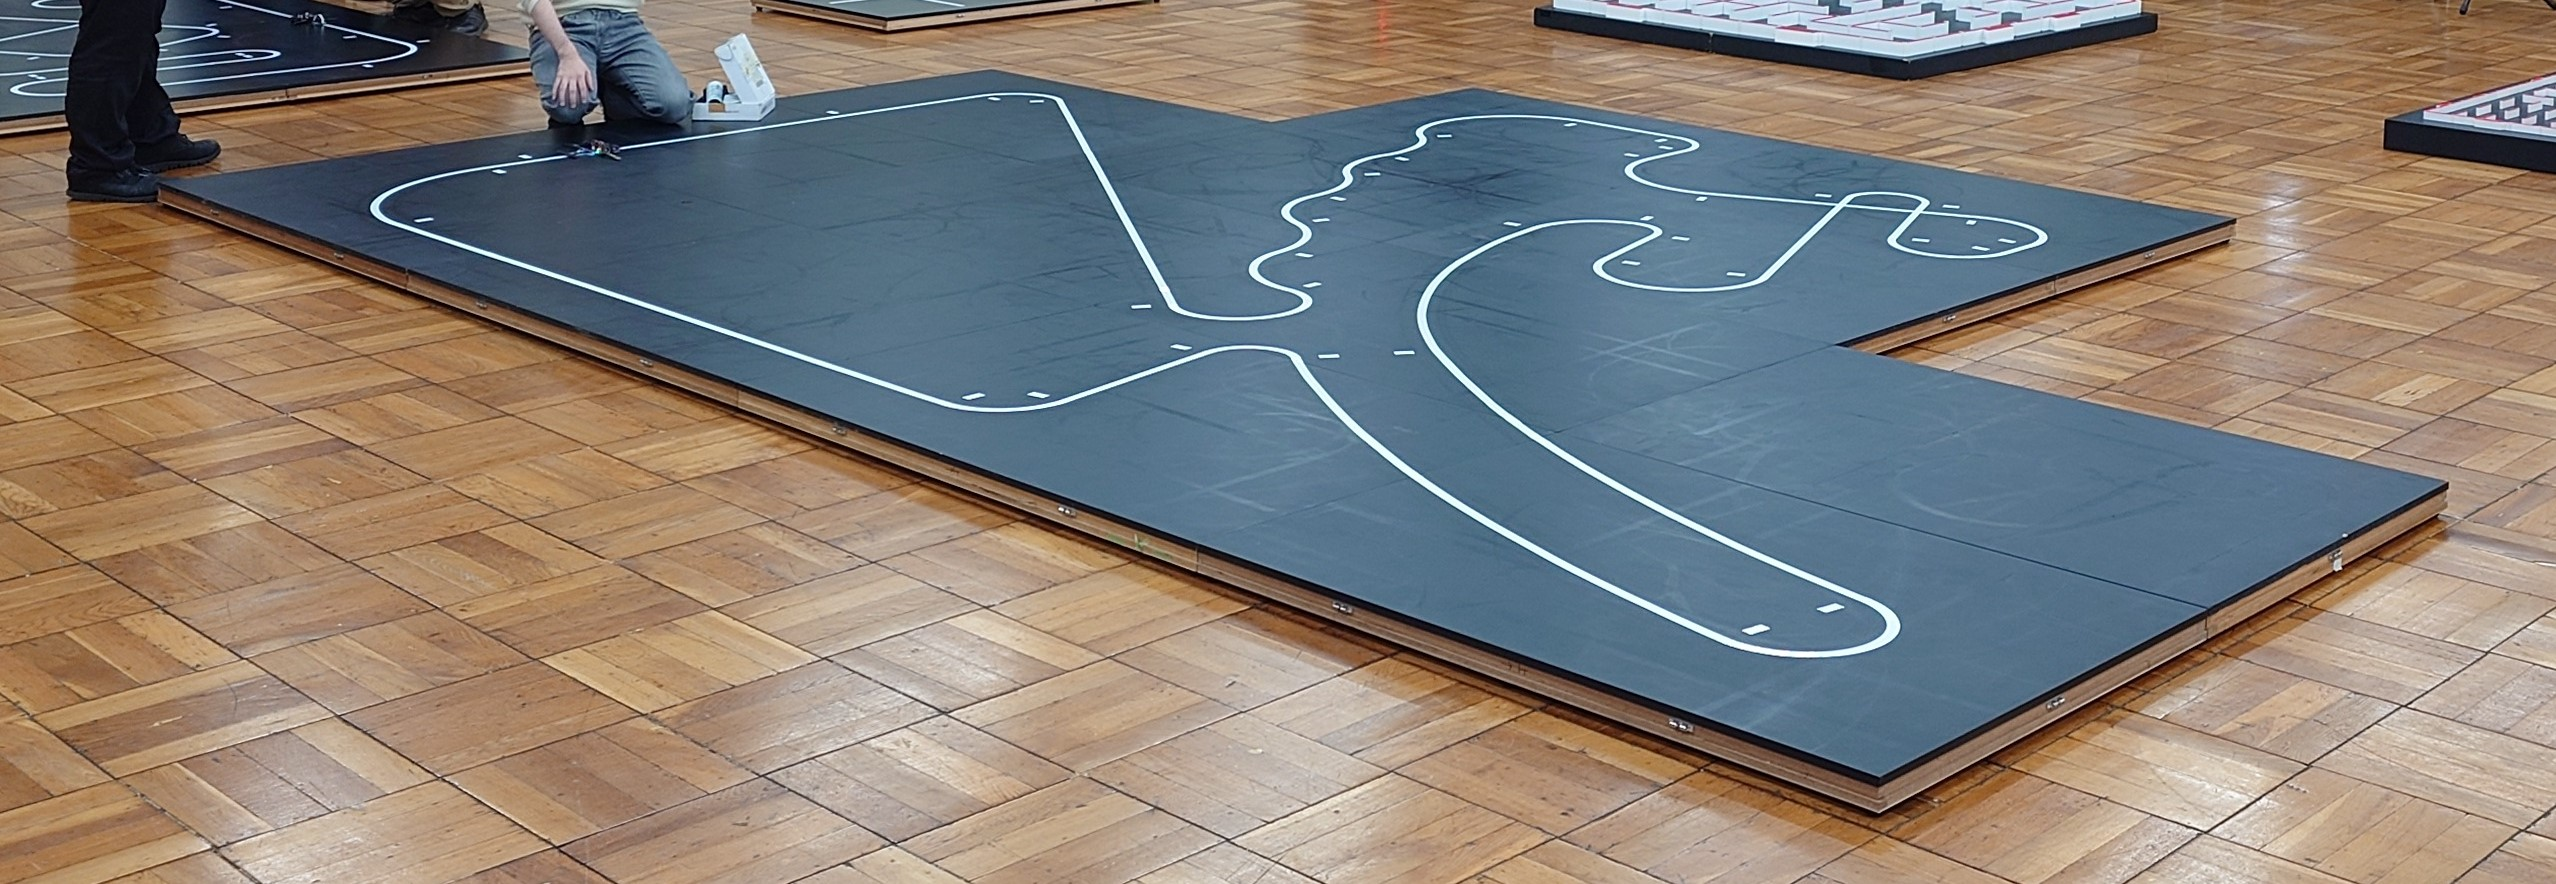
\includegraphics[width=0.8\textwidth]{ejemplo_pista_1}
\caption{\label{fig:pista1} Ejemplo de pista} Fuente: Elaboración propia.
\end{figure}

Los últimos años todos los esfuerzos de mejora se han enfocado en la mecánica y electrónica del robot, principalmente con la adición de métodos de succion mediante turbinas, dejando de lado el software. Es por este motivo que en la última versión no se ha otorgado el premio a la innovación a ningún participante.

\subsection{Arquitectura Actual}
En la última competencia realizada, la gran mayoría (por no decir todos), programaba sus robots en C/C++, aplicando algoritmos de MATLAB (más adelante se detalla). La ventaja de esto es que MATLAB genera scripts en C/C++, por lo que se pueden usar algoritmos de optimización preexistentes sin mayores complicaciones.

\subsubsection{Mapeo}
Para la primera vuelta, los robots deben ser capaces de las siguientes 2 características: identificar las marcas de curva que se encuentran en la pista en cada cambio de curvatura (Ver figura \ref{fig:marcaspista}) y poder saber su posición actual en términos de coordenadas cartesianas (x,y).

\begin{figure}[h]
\centering
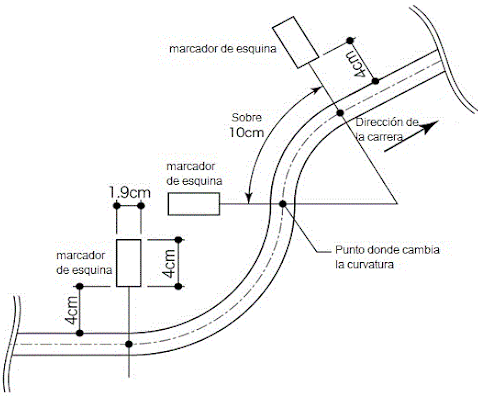
\includegraphics[width=0.8\textwidth]{ejemplo_marcas_curvas}
\caption{\label{fig:marcaspista} Ejemplo de marcas de curva} Fuente: All Chile Robot Contest.
\end{figure}

Para la primera, se necesitan sensores infrarrojos capaces de identificar blanco vs negro posicionados de tal forma que siempre detecten las marcas correspondientes. Para la segunda se pueden utilizar 2 elementos de manera independiente o junta (esta última es la más óptima): Encoders en cada rueda (Odometría), lo cual permite saber la velocidad real de cada una. Y una IMU , que básicamente es un giroscopio+acelerómetro.

De esta forma se puede hacer una estimación relativamente precisa de la posición del robot en términos de (x,y), resultando en una nube de puntos que representan la pista. Usualmente esta información es guardada en un simple txt.

\subsubsection{Optimización}
Con la nube de puntos generada, se utiliza un algoritmo de MATLAB conocido como PRM\footnote{\url{https://la.mathworks.com/help/robotics/ug/probabilistic-roadmaps-prm.html} , PRM algorithm.}, en donde se define 
un mapa binario donde la ruta generada, más el ancho del robot, se define como espacio válido para desplazarse, y el resto como obstáculo. Luego se generan puntos aleatorios dentro de la zona donde el robot puede pasar y finalmente se juntan los que permiten la ruta más corta posible(Ver figura \ref{fig:PRM}).

\begin{figure}[h]
\centering
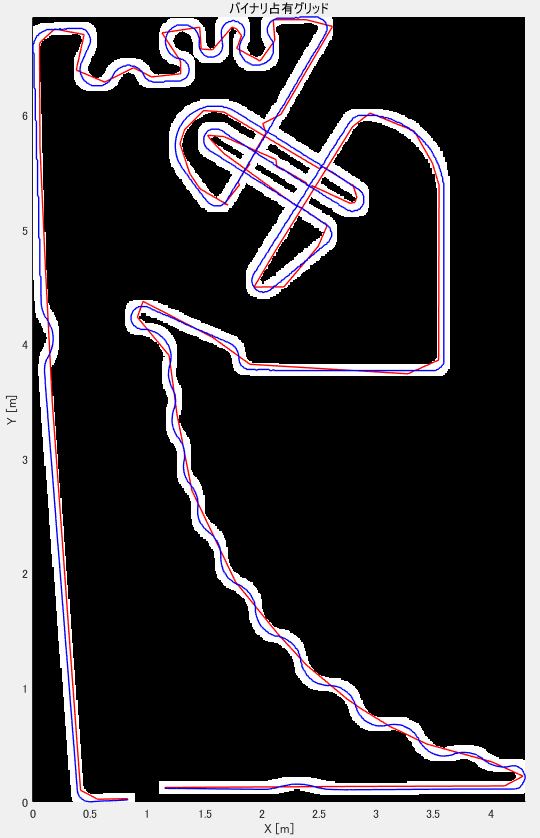
\includegraphics[width=0.5\textwidth]{ejemplo_optimizacion_PRM}
\caption{\label{fig:PRM} Aplicación de PRM} Fuente: Haruki Shimotori.
\end{figure}

\newpage
Con la ruta definida, mediante un algoritmo de seguimiento de rutas \footnote{\url{https://la.mathworks.com/help/robotics/ug/path-following-for-differential-drive-robot.html} , Path follower}, se le dan las instrucciones de movimiento al robot, donde en cada intento se varían las variables de velocidad, aceleración y freno.

Esta información fue basada en las publicaciones de Haruki Shimotori \footnote{\url{https://underbirdworks.blogspot.com/2020/12/matlabprm.html}, explicacion de Haruki Shimotori } y en el siguiente video se puede ver una idea similar en donde se utiliza Path Smoothing \cite{pathsmoothing}


\newpage
\secnumbersection{MARCO CONCEPTUAL}

Los fundamentos teóricos necesarios para fundamentar el aspecto de software consta de los siguientes elementos:
\begin{itemize}
\item Redes neuronales
\item Redes convulocionales
\item Visión computacional
\item Aprendizaje reforzado
\end{itemize}

Por otro lado, si bien no es el enfoque de este trabajo, es necesario entender los siguientes conceptos complementarios:
\begin{itemize}
\item Raspberry Pi
\item Robotic Operating System (ROS)
\item Control diferencial de motores
\item Simulador Webots
\end{itemize}
\newpage
\input{propuesta_de_solucion}
\newpage
\input{validacion_de_la_solucion}
\newpage
\input{conclusiones}

\newpage
\secnumberlesssection{ANEXOS}

\begin{figure}[h]
\centering
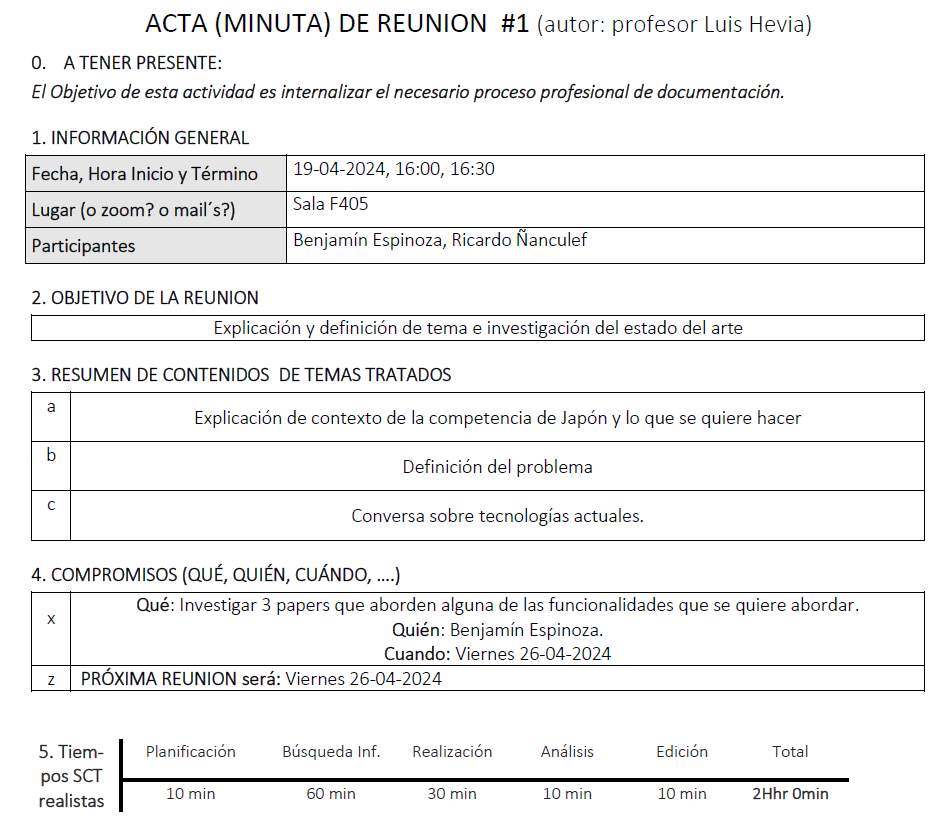
\includegraphics[width=1\textwidth]{minuta_reunion}
\caption{\label{fig:Minuta1} Minuta de reunion con profesor guía} Fuente: Elaboración propia.
\end{figure}



\newpage
% Bibliografía estilo APA:
\bibliographystyle{apalike-es}
\bibliography{bibliografia}{}

\end{document}
